% -*- root: cuthesis_masters.tex -*-

In this chapter we will present related work on technical debt. These studies sets the current background of technical debt. More specifically, the studies presented in this chapter are three fold. First, we present studies that discuss the definition and the extensibility of the technical debt metaphor. This first part lays the foundation of what it is technical debt and how it is being used nowadays. Second, we present studies that investigate the identification and the implications of technical debt in the source code. Third we present the studies that are more related with our own work which is the identification of \emph{self-admitted} technical debt. 

Although we provide a broad review of related work in technical debt in this chapter, more specific related work can be found in the chapters \ref{chapter3} and \ref{chapter4}.

\section{Defining and Expanding the Technical Debt Metaphor}
\label{defining_and_extending_technical_debt}

At first, most information about technical debt were available on blogs. These blogs were written by industry specialists and evangelists of Agile Methodologies, such as Martin Fowler. Nowadays, academia and industry alike study the applications of the technical debt metaphor. Thus, a large number of studies were dedicate to this matter, and therefore, the original metaphor has been expanded and refined.

The metaphor \textit{technical debt} was introduced by Ward Cunningham~\cite{Cunningham1992WPM} more than two decades ago to facilitate the communication between developers and non-technical personal working on the same software project. Cunningham explains how ``not quite right code'' will affect the maintainability of a project (i.e., require more effort to maintain the project in the future) as interest does on incurred debt. 

In other words, every time that a implementation around the code affected by the non-optimal implementation is needed, an interest in form of effort will be expend in the task. Although debts may speed up the project development at first, accumulated debt will bring the project to a standstill in the long-run. Thus, the technical debt metaphor, provide insight to managers of why it is beneficial to use resources to enhance a particular portion of the code even if it is not broken.

The term has been refined and expanded since, notably by Steve McConnell~\cite{McConnell07:TechnicalDebt} in his taxonomy and by Martin Fowler~\cite{MartinFowler:TechnicalDebtQuadrant} with his four quadrants. As these works were very important to the development of a deeper understanding of technical debt and its applicability on software engineering we dedicated subsections \ref{chap2:mcconnel_subsection} and \ref{chap2:fowler_subsection} for further explanation on the authors' definition of technical debt. 

\subsection{Unintentionally incurred debt vs. Intentionally incurred debt}
\label{chap2:mcconnel_subsection}

According to Steve McConnell, technical debt can be divided into two main kinds: \textit{unintentionally incurred debt} and \textit{intentionally incurred debt}.

Examples of unintentionally incurred debt ranges from a design approach that just turns out to be error-prone to a junior programmer who  write bad code. This technical debt is the non-strategic result of doing a poor job. In some cases, this kind of debt can be incurred unknowingly, for example, when a company acquire another company that has accumulated technical debt over the years. 

The second kind of technical debt, incurred intentionally, commonly occurs when an organization makes a conscious decision to optimize for the present rather than for the future. An ``If we do not get this release done on time, there will not be a next release'' type of situation. This leads to decisions like, ``We do not have time to reconcile these two databases, so we will write some glue code that keeps them synchronized for now and reconcile them after we ship.'' Or ``We have some code written by a contractor that does not follow our coding standards; we will clean that up later.'' Or ``We did not have time to write all the unit tests for the code we wrote the last 2 months of the project. We'll right those tests after the release''. 

Moreover, technical debt incurred intentionally can be of two types: short-term and long term debt. Like with real debt, short-term debt is expected to be paid off frequently. Short-term debt is taken on tactically and reactively, usually as a late-stage measure to get a specific release out the door, whereas long term debt is taken on strategically and pro-actively. For example, ``We do not think we are going to need to support a second platform for at least five years, so this release can be built on the assumption that we are supporting only one platform''.

The implication is that short-term debt should be paid off quickly, perhaps as the first part of the next release cycle, whereas long-term debt can be carried for a few years or longer.

Therefore, McConnell presents the following \textbf{taxonomy for technical debt} to summarize his thoughts on technical debt:

\begin{enumerate}
    \item - Debt incurred \textbf{unintentionally} due to low quality work
    \item - Debt incurred \textbf{intentionally}
    \begin{enumerate}
        \item - \textbf{Short-term debt}, usually incurred reactively, for tactical reasons
        \begin{enumerate}
            \item - Focused Short-Term Debt. Individually identifiable shortcuts (like a car loan)
            \item - Unfocused Short-Term Debt. Numerous tiny shortcuts (like credit card debt)
        \end{enumerate}
        \item - \textbf{Long-term debt}, usually incurred pro actively, for strategic reasons
    \end{enumerate}
\end{enumerate}

\subsection{Technical Debt Quadrant}
\label{chap2:fowler_subsection}

On the other hand, Fowler definition of technical debt is slight different, and it is represented by four quadrants namely reckless, prudent, deliberate and inadvertent. According to Fowler debt can be any combination of these four quadrants. 

For example, prudent deliberate debt is the one that the team knows they are taking on a debt, and thus puts some thought as to whether the payoff for an earlier release is greater than the costs of paying it off. However, a team not aware of design practices is taking on its reckless debt without even realizing how much hack it's getting into (inadvertent). Although reckless debt may not be inadvertent. A team may know about good design practices, but decide to go ``quick and dirty'' because they think they can not afford the time required to write clean code. The fourth cell of the quadrant is prudent/inadvertent debt. This case represent the case where a skilled development team is creating a project applying the best design to handle the current requirements, however over time, the chosen design proves to be inadequate to the future need of the project. Fowler points out that the point is that while you are programming, you are also learning. It is often the case that it can take a year of programming on a project before you understand what the best design approach should have been.  

 
\begin{figure*}[thb!]
  \centering
  \vspace{5mm}
  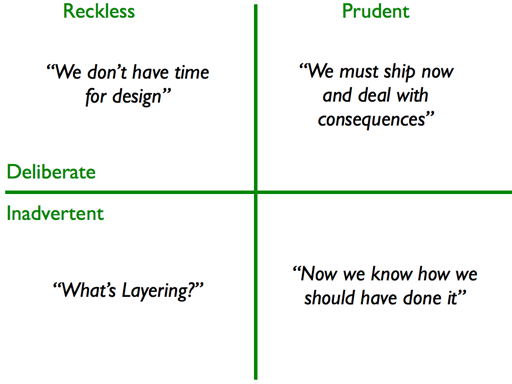
\includegraphics[width=.65\textwidth]{figures/literature_review/technical_debt_quadrant.png}
  \caption{Technical Debt Quadrant}
  \label{fig:technical_debt_quadrant}
\end{figure*}


Figure \ref{fig:technical_debt_quadrant} presents the actual technical debt quadrant, and illustrates on each cell the possible cases that can happen with a development team while working on a software project. 

In addition, from the original description ``\textit{not quite right code which we postpone making it right}'' various people have used the metaphor of technical debt to describe many other \emph{kinds} of debts or faults of software development, including anything that is related to deploying, selling, or evolving a software system or anything that is intrinsic to software development such as test debt, people debt, architectural debt, requirement debt, documentation debt, or just an broad generalized software debt \cite{sterling2010book}. 

In this matter, Kruchten \textit{et al.}~\cite{kruchten2012IEEE} express their concern about how the use (or abuse) of the metaphor could spread it too thin making the metaphor lose its communication power. For example, a not yet implemented requirement, function, or feature does not translate to  requirement debt. Similarly, postponing the development of a new function is not a planning debt. Another danger pointed out by the authors relates to the assistance of static code analyzers tools on the identification of technical debt. Although these tools are very useful there is a danger of equating whatever the tools can detect with what is technical debt. This approach leads to leaving aside large amounts of potential technical debt that is undetectable by tools, such as structural or architectural debt, technological gaps or self-admitted technical debt as discussed later on this chapter. 

Later, Spinola \textit{et al.} \cite{Spinola2013MTD} identified and organized a number of statements about technical debt expressed by practitioners in online websites, blogs and published papers. The authors chose 14 statements related to technical debt and conducted two surveys with 37 participants to evaluate the level of agreement on each statement. 
They found that practitioners strongly agree that if technical debt is not managed effectively, maintenance costs will increase at a rate that will eventually outrun the value it delivers to customers. In addition, they found that practitioners strongly disagree that all technical debt is intentional, the results found by the authors support the expanded technical debt definition proposed by McConnel and Fowler. 

Moreover, the authors state that the acceptance and use of the TD metaphor is in large part because it is easily understood. However, this can also be a concern to accurately define technical debt. Their reasoning is that because the TD metaphor is easy to understand, it is also easy to talk about, expand on, and relate experience to. A quick search of TD literature reveals subjective opinions, personal views, and catch phrases on such channels as blogs and online essays. Therefore, more analysis on the use of the metaphor is necessary to organize the technical debt landscape.

Alves \textit{et al.}~\cite{Alves2014MTD,Alves2016IST} proposes an ontology of terms on technical debt in order to organize a common vocabulary for the area. In their work they extracted and organized concepts derived from the results of a systematic literature mapping. In total, 100 studies, dated from 2010 to 2014, were evaluated. Their work contributed towards the evolution of the technical debt landscape through the organization of the different types of technical debt and their indicators. The authors found in the literature the following types of debt: design debt, architecture debt, documentation debt, test debt, code debt, defect debt, requirements debt, infrastructure debt, people debt, test automation debt, process debt, build debt, service debt, usability debt and versioning debt. Moreover, they state that some instances of technical debt can fit more than one type of technical debt. 

These works summarize the definition and expansion of the technical debt metaphor. 

\subsection{Identification and Implications of Technical Debt in the Source Code}

A number of studies have focused on the detection and management of technical debt. Much of this work has been driven by the Managing Technical Debt Workshop community. 






% A number of studies has focused on the detection and management of technical debt. For example, Seaman et al. [SG11], Kruchten et al. [KNOF13] and Brown et al. [BCG+10] make several reflections about the term technical debt and how it has been used to communicate the issues that developers find in the code in a way that managers can understand.
% 62
% Other work focused on the detection of technical debt. Zazworka et al. [ZSV+13] conducted an experiment to compare the efficiency of automated tools in comparison with human elicitation regarding the detection of technical debt. They found that there is a small overlap between the two approaches, and thus it is better to combine them than replace one with the other. In addition, they concluded that automated tools are more efficient in finding defect debt, whereas developers can realize more abstract categories of technical debt.

% In a follow up work, Zazworka et al. [ZSSS11] conducted a study to measure the im- pact of technical debt on software quality. They focused on a particular kind of design debt, namely, God Classes. They found that God Classes are more likely to change, and therefore, have a higher impact on software quality. Fontana et al. [FFS12] inves- tigated design technical debt appearing in the form of code smells. They used metrics to find three different code smells, namely God Classes, Data Classes and Duplicated Code. They proposed an approach to classify which one of the different code smells should be addressed first, based on its risk. Ernst et al. [EBO+15] conducted a survey with 1,831 participants and found that architectural decisions are the most important source of technical debt.

